
\documentclass[11pt]{article}
\usepackage{amsmath,amssymb,amsfonts} 
\usepackage{epsfig} \usepackage{latexsym,nicefrac,bbm}
\usepackage{xspace}
\usepackage{color,fancybox,graphicx,subfigure,fullpage}
\usepackage[top=1.25in, bottom=1.25in, left=1in, right=1in]{geometry}
\usepackage{tabularx} \usepackage{hyperref} 
\usepackage{pdfsync}
\usepackage[boxruled]{algorithm2e}
\usepackage{multicol}
\usepackage{enumitem}
\newcommand{\parag}[1]{ {\bf \noindent #1}}
\newcommand{\defeq}{\stackrel{\textup{def}}{=}}
\newcommand{\nfrac}{\nicefrac}
\newcommand{\opt}{\mathrm{opt}}
\newcommand{\tO}{\widetilde{O}}
\newcommand{\polylog}{\mathop{\mbox{polylog}}}
\newcommand{\supp}{\mathrm{supp}}
\newcommand{\rank}{\mathrm{rank}}
\newcommand{\ptot}{p_{\mathrm{tot}}}
\newcommand{\pmin}{p_{\mathrm{min}}}
\newcommand{\pmax}{p_{\mathrm{max}}}
\newcommand{\prob}[1]{\mathrm{Pr}\insquare{#1}}


\newcommand{\conv}{\mathrm{conv}}
\newcommand{\dist}{\mathrm{dist}}
\newcommand{\argmin}{\operatornamewithlimits{argmin}}
\newcommand{\sgn}{\mathrm{sgn}}
\newcommand{\fc}{\mathrm{fc}}


\newcommand{\cM}{\mathcal{M}}
\newcommand{\cB}{\mathcal{B}}
\newcommand{\cU}{\mathcal{U}}
\newcommand{\cY}{\mathcal{Y}}
\newcommand{\cF}{\mathcal{F}}
\newcommand{\capa}{\mathrm{Cap}}
\newcommand{\dcapa}{\underline{\mathrm{Cap}}}
\newcommand{\st}{\mathrm{s.t.}}
\newcommand{\un}{\mathrm{un}}

\newcommand{\Pb}{\mathbb{P}}
\newcommand{\sym}{\mathrm{sym}}
\newcommand{\pcount}{\mathbf{PCount}}
\newcommand{\mixdet}{\mathbf{MixDisc}}
\newcommand{\sbold}{\mathbf{S}}
\newcommand{\mb}{{M(\cB)}}

\newcommand{\mlb}{{M_{\mathrm{lin}}(\cB)}}
\newcommand{\redc}[1]{ \textcolor{red} {#1}}
\newcommand{\newt}{\mathrm{Newt}}
\newcommand{\wtf}{\widetilde{f}}
\newcommand{\wt}{\widetilde}
\newcommand{\diam}{\mathrm{diam}}
\newcommand{\lspan}{\mathrm{span}}
\newcommand{\interior}{\mathrm{int}}
\newcommand{\aff}{\mathrm{aff}}
\newcommand{\per}{\mathrm{per}}
\newcommand{\bl}{\mathrm{BL}}
\newcommand{\cE}{\mathbb{E}}


\newcommand{\eps}{\varepsilon}

\newenvironment{proof}{\noindent{\bf Proof:}\hspace*{1em}}{\qed\bigskip}
\clubpenalty=10000
\widowpenalty = 10000
\newcommand{\qed}{\hfill\ensuremath{\square}}


\def\showauthornotes{0} 
\def\showkeys{0} 
\def\showdraftbox{0}


\newcommand{\Snote}{\Authornote{S}}
\newcommand{\Scomment}{\Authorcomment{S}}

\newcommand\Z{\mathbb Z}
\newcommand\N{\mathbb N}
\newcommand\R{\mathbb R}
\newcommand\C{\mathbb C}

\newtheorem{theorem}{Theorem}[section]
\newtheorem{fact}{Fact}[section]
\newtheorem{conjecture}[theorem]{Conjecture}
\newtheorem{definition}{Definition}[section]
\newtheorem{lemma}[theorem]{Lemma}
\newtheorem{remark}[theorem]{Remark}
\newtheorem{proposition}[theorem]{Proposition}
\newtheorem{corollary}{Corollary}[section]
\newtheorem{claim}[theorem]{Claim}

\newtheorem{openprob}[theorem]{Open Problem}
\newtheorem{remk}[theorem]{Remark}
\newtheorem{example}[theorem]{Example}
\newtheorem{apdxlemma}{Lemma}
%\newtheorem{algorithm}[theorem]{Algorithm}
\newcommand{\question}[1]{{\sf [#1]\marginpar{?}} }

%% probability stuff

\newcommand\pr{\mathop{\mbox{\bf Pr}}}
\newcommand\av{\mathop{\mbox{\bf E}}}
\newcommand\var{\mathop{\mbox{\bf Var}}}

\newcommand{\ex}[1]{\av\left[{#1}\right]}
\newcommand{\Ex}[2]{\av_{{#1}}\left[{#2}\right]}

\def\abs#1{\left| #1 \right|}
\newcommand{\norm}[1]{\ensuremath{\left\lVert #1 \right\rVert}}



\newcommand{\tr}[1]{\mathop{\mbox{Tr}}\left({#1}\right)}
\newcommand{\diag}[1]{{\sf Diag}\left({#1}\right)}

\newcommand\set[1]{\left\{#1\right\}} %usage \set{1,2,3,,}
\newcommand{\poly}{\mathrm{poly}}
\newcommand{\floor}[1]{\left\lfloor\, {#1}\,\right\rfloor}
\newcommand{\ceil}[1]{\left\lceil\, {#1}\,\right\rceil}
\newcommand{\comp}[1]{\overline{#1}}
\newcommand{\pair}[1]{\left\langle{#1}\right\rangle} %for inner product
\newcommand{\smallpair}[1]{\langle{#1}\rangle}

\newcommand{\inparen}[1]{\left(#1\right)}             %\inparen{x+y}  is (x+y)
\newcommand{\inbraces}[1]{\left\{#1\right\}}           %\inbrace{x+y}  is {x+y}
\newcommand{\insquare}[1]{\left[#1\right]}             %\insquare{x+y}  is [x+y]
\newcommand{\inangle}[1]{\left\langle#1\right\rangle} %\inangle{A}    is <A>


\newenvironment{proofsketch}{\begin{trivlist} \item {\bf
Proof Sketch:~~}}
  {\qedsketch\end{trivlist}}

\newenvironment{proofof}[1]{\begin{trivlist} \item {\bf Proof
#1:~~}}
  {\qed\end{trivlist}}


\title{\bf CPSC 464: Modeling Alternative Affordable Housing Priority Systems}


\author{Andrew West, Nicole Lam, Atul Pokharel, Urszula Solarz \\
Professor: Nisheeth K. Vishnoi
}





\begin{document}


\maketitle
 
\begin{abstract}

Write a 6-8 line abstract clearly stating the high level goals and the concrete desired goals of this project. 
  
\end{abstract}


\newpage



\tableofcontents

\newpage

\section{Introduction}

\paragraph{High level description of the problem.}

\paragraph{Motivation to study the problem.}

\paragraph{Most related prior works.}
Explain in detail the most related (around 3) prior works. For each, 

\begin{enumerate}
\item  mention how they address the high level problem mentioned above,

\item in what ways do they succeed and what are their positives, and

\item in what ways are they insufficient.

\end{enumerate}




\paragraph{Desired contributions.}
Write down a bullet list of desired contributions that emphasize:

\begin{itemize} 

\item Conceptual novelty (e.g. first attempt to study the problem, new model, etc.)

\item Technical novelty (e.g. a new theorem)

\item Novelty in proofs (leave blank if not done yet or not applicable)

\item Empirical evaluations: 1) on simulated datasets, 2) real-world datasets.

\end{itemize}

\paragraph{Feasibility and potential risks.}


\section{Other related works}

The allocation of scarce resources is a classic problem that pervades social service delivery. At the highest level, prior research has examined the necessity of trade-offs for fairness in social contexts \cite{mashiat2022trade}, arguing that often times many reasonable definitions of equity cannot hold simultaneously. This paper in particular creates a metric of fairness to analyze average realized utility of a resulting outcome, but does not give way to implement allocation systems, which we wish to examine. \\

\newline
There are a variety of studies regarding affordable housing and approximating allocation algorithms. The major limitation of all these studies is that the algorithms are not public. However, Figure 1 describes the general stages of any scheme.\\
\newline
Some papers have abstracted the problem of housing allocation into that of designing waitlists and lotteries \cite{arnosti2020design}. They claim that two approaches of housing allocation create near-optimal matches: independent lotteries and waitlists. They examine in great detail these two modes of allocation, but does not examine the inherent factor of consumer choice in the housing allocation process. Another paper addresses this shortfall by implementing a modified version of the latter of these systems on housing data from Pittsburgh \cite{harvardpublichousing}. Specifically addressing the issue of allocation inefficiency, they argue that implementing an independent waitlist per building reduces the amount of vacant buildings emptied during turnover. However, this algorithm does not account for the nuances of household differences (size, number of children/elderly, veteran status...), which is what we intend to explore. \\

\newline

In our project, we aim to analyze the demographic effects of tenant populations by changing the order of allocations, as in \cite{nyuaffordablehousing}. This paper tackles the issue that housing allocation methods are often unknown and opaque. Thus, they created an algorithm to include priority systems (moving populations with certain characteristics to the front of a queue). Specifically, they analyzed the changes in tenant composition by prioritizing high income households, low income households, the elderly population, and families with children under 18. While the model does shed light on the magnitude of change in these particular orderings, it limits the eligible applicants to those whose household income is above 80\% of the area median income, which severely skews the results. There are also many other key variables such as families with victims of domestic violence, military status, and veteran status that were not explored.\\




\section{The Model/Framework}
\noindent
Our city of choice to model policy changes is Baltimore. With a population of close to 600,000 and a public housing system containing approximately 6,000 properties, Baltimore's robust and widely used public housing system is an ideal choice for analyzing the impacts of differing priority systems on allocation outcomes. \\
\newline
Demand for public housing in Baltimore is also exceedingly high. The public housing system lottery opened for the first time since 2019 this August, with nearly 30,000 applicants applying during the two week window. (source: https://www.wypr.org/wypr-news/2023-08-14/28-000-apply-for-baltimore-city-housing-wait-list-two-week-window-ends-tonight). Priority systems are unfortunately essential to best allocate the limited available housing to those most in need. \\
\newline
Baltimore is also an ideal choice due to the availability of relevant datasets, discussed further in 6.1. \\
\newline 
Our model includes multiple components due to the complexity of applicant selection that takes place in public housing allocation. Broadly, the framework is as follows:
\begin{enumerate}
    \item Estimate who is eligible for Baltimore public housing, and of the eligible pool, who applies.
    \item Estimate the existing allocation system.
    \item Implement changes in housing priority systems and model the effects when compared to actual waitlist demographics. 
\end{enumerate}
Modeling the waitlist and how it changes under new policies also requires us to consider the human factors that impact waitlist membership. In particular, we will make assumptions about the rate at which applicants apply, any applicants that leave the waitlist, and the rate at which apartments become available for new occupants.
\subsection{Various Housing Allocation Algorithms}
As forementioned in our prior related works section, we know very little about the methods jurisdictions use to allocate assistance. One such paper attempts to approximate the different algorithms of housing allocation systems deployed in different cities. The steps are detailed below:
\begin{enumerate}
    \item Housholds successfully complete the application for housing assistance. Many eligible housholds don't apply for assitance due to lack of functioning abilities, language skills, or other tools needed to complete the application.
    \item Applications are deemed eligible or non-eligible (i.e. some cities only allow those with income greater than 80\% of average median income to apply)
    \item Categorize the various characteristics for each household applicant (unit size, military status, number of children, income level, etc.)
    \item Match type of housing (1-bedroom, 2-bedroom, etc.) with each household applicant based on their characteristics in step 3
    \item The order in which applicants will receive allocations for each housing type is determined (i.e. lottery, queue, waiting list, some metric of ``need", or a combination)
    \item Present chosen applicants with at least one housing option. In some cases, applicants apply only for a particular housing development in some location, so they must take the option or leave the queue (or allocation system) all together. Other systems allow applicants to reject the particular unit or development, but stay in the queue for other, more desirable, units that become available.
\end{enumerate}
\subsection{Cambridge Housing Model}
\label{sec:chm}
In the same paper, the author attempts to examine the specific housing system of one Public Housing Agency: the Cambridge, MA Public Housing Agency (CHA) at a specific point in time (2012 calendar year) \cite{nyuaffordablehousing}. First, the paper approximates the allocation algorithm.

\section{(Desired) Theoretical results}


\subsection{Preliminary results}


\section{(Desired) Empirical results}

\subsection{Setup}
\paragraph{Datasets.}
Our work will employ three datasets. The first is the \textit{American Community Survey (ACS) microdata} (source: https://data.census.gov/mdat/\#/search?ds=ACSPUMS5Y2021). The ACS is an annual survey conducted with the aim of being a nationally representative sample of demographic, economic, and housing information. We will employ demographic variables contained in the ACS data to estimate the number of households elligible for public housing. \\
\newline
Our second dataset is the \textit{HUD’s Picture of Subsidized Households (PIC) data} (source: https://www.huduser.gov/portal/datasets/assthsg.html). The PIC data contains information on demographics of public housing tenants, public housing vacancy rates, and average waiting times that will be helpful in constructing our model. \\
\newline
Finally, we will make use of the \textit{2020 Baltimore public housing waiting list demographics} (source: https://www.hud.gov/sites/dfiles/PIH/documents/BaltimoreFY20Report.pdf). This information will allow us to validate our model of the existing allocation system.

\paragraph{Algorithms}

Using the Cambridge housing allocation model in section~\ref{sec:chm}, we will simulate the waitlist most likely in C. Each simulation 

\paragraph{Baselines and metrics}



\subsection{Preliminary results}


\section{Conclusion, limitations, and future Work}
Discuss the importance of the results, state the limitations, and point out avenues of future work/open problems.
\newpage
\section{Data Prep Scripts}
.do files prepare the data. Filenames in bold are not generated by the scripts. They have to be available to them instead. Each of the scripts is described below.

\subsection{ACS-extract.do}
Input: \textbf{data/ACS/usa\_00003.dat/usa\_003.dat} \\
Output: data/ACS\_2006\_2017.dta \\
Guess: This looks like American Community Survey (ACS) data from 2006 to 2017. \\
Source: 

\subsection{descriptives-CHA.do}
Input: data/Matlab/eligible\_population\_CHA.dta \\
Output:  results/Descriptive/ \\
- acs\_descriptive\_CHA.dta \\
- descriptive\_table\_auto.xls  (with sheets “ACS All”, “ACS by Type” )\\
		- acs\_descriptive\_CHA\_bytype.dta\\
		- pic\_descriptive\_CHA.dta\\
		- descriptive\_table\_auto.xls ( with sheet "PIC All" and "PIC by Type" )\\
		- pic\_counts\_CHA\_bytype.dta\\

\subsection{eligible-population.do}
Input: data/\\
ACS/ACS\_2006\_2017.dta\\
\textbf{other/ami.dta}\\
Output: data/Matlab/ \\
- eligible\_population\_CHA.dta\\
- eligible\_population\_CHA.txt (A pipe delimited file)

\subsection{pic-data.do}
Input: data/ \\
\textbf{HUD-PIC/2012/PROJECT\_2012.csv} \\
\textbf{other/CHA-projects.csv} \\
Output: \\
data/ \\
- HUD-PIC/2012/PIC-CHA.dta \\
- Matlab/projects-ready.dta \\
- Matlab/projects-ready.txt \\
- other/waiting-times-CHA.dta\\
results/descriptive/ \\
-   pic\_by\_development.dta \\
- development\_characteristics.xls ( with sheet("raw") ) \\

\section{Primary Datasets}
The data processing pipeline is shown in Figure~\ref{fig:datapipeline}. The primary files are underlined in red  and described below. See the associated  spreadsheet for the fields and below for any additional notes.

\begin{figure}
    \centering
    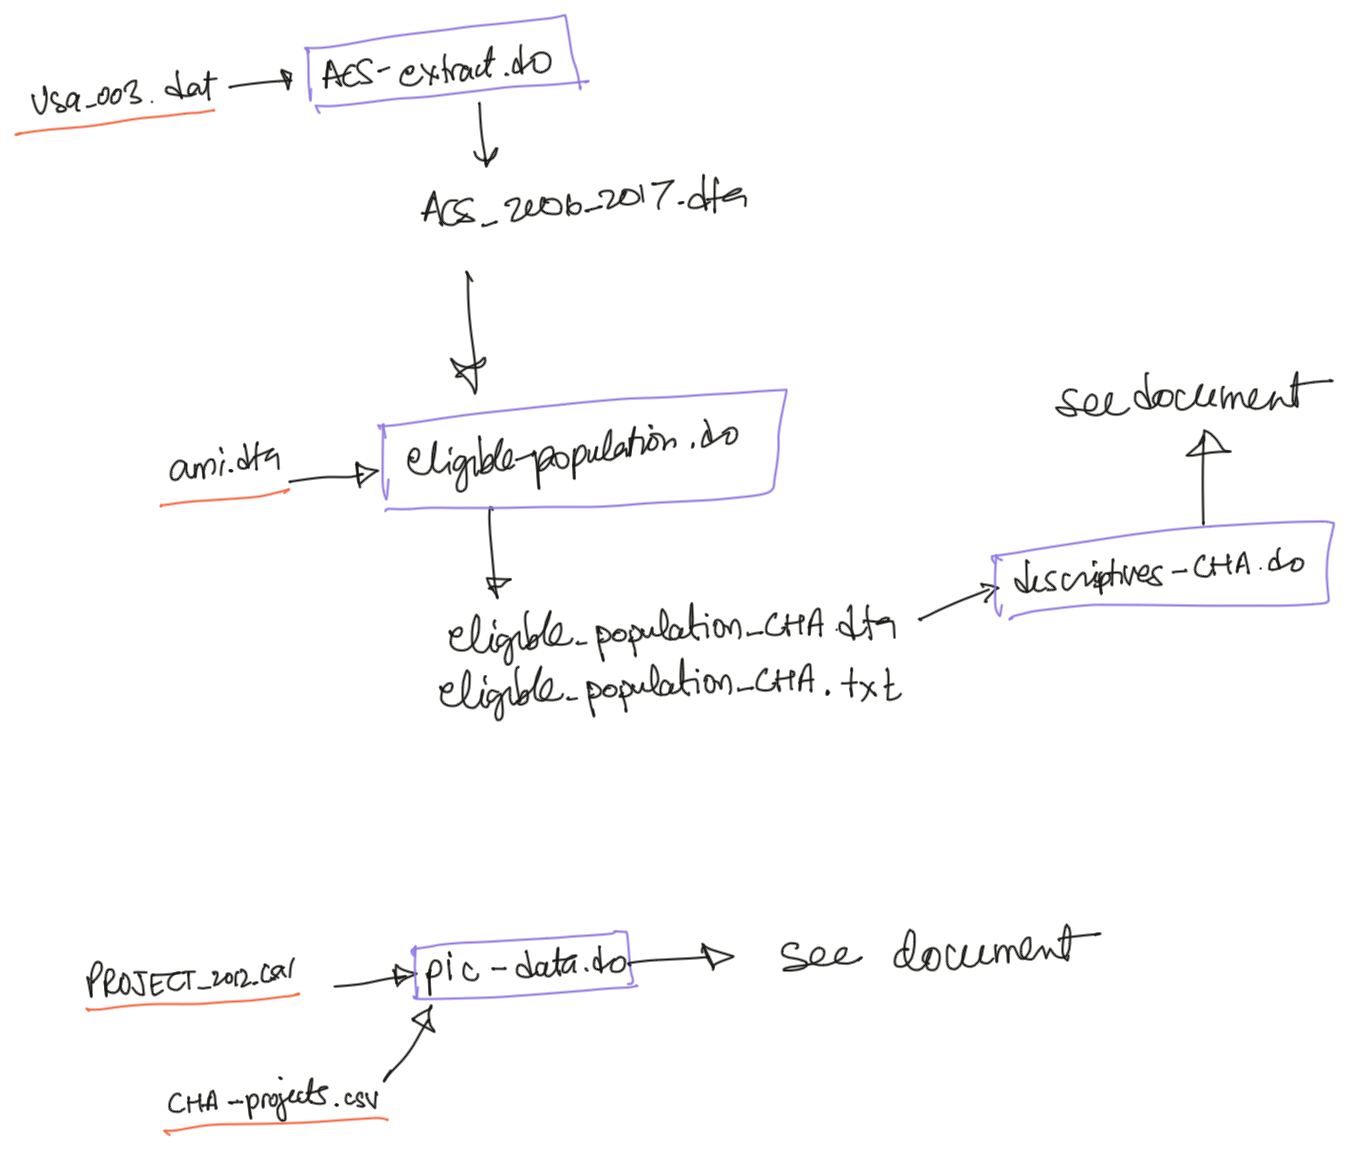
\includegraphics[width=1\linewidth]{doc/data_processing_pipeline.png}
    \caption{Data processing pipeline. Primary data is underlined, and scripts are in purple boxes. Arrows denote input or output.}
    \label{fig:datapipeline}
\end{figure}


\subsection{usa\_003.dat}

\subsection{ami.dta}

\subsection{PROJECT\_2012.csv}

\subsection{CHA-projects.csv}

\section{Analysis Scripts}
.m files primarily run simulations and analysis on the data. 
\bibliographystyle{plain}
\bibliography{doc/references} 


\end{document}
